\documentclass{article}
\usepackage{listings}
\usepackage[utf8]{inputenc}
\usepackage{graphicx}
\usepackage{subfiles}
\usepackage{wrapfig}
\usepackage{geometry}
\usepackage[italian]{babel}
\usepackage[export]{adjustbox}
\usepackage[font=scriptsize]{caption}
\usepackage{titlesec}
\usepackage{amsmath}
\usepackage[titletoc]{appendix}

\setcounter{section}{-1}
\hyphenation{ bottleneck }



\titlespacing*{\section}
{0pt}{3ex plus 1ex minus .2ex}{3ex plus .2ex}
\titlespacing*{\subsection}
{0pt}{3ex plus 1ex minus .2ex}{3ex plus .2ex}
\graphicspath{ {./images/} }
\geometry{a4paper, top=2cm, bottom=2cm, left=2cm, right=2cm, heightrounded, bindingoffset=5mm}

\title{\Huge LABORATORIO DI INTERNET 
    \\ Tesina di gruppo \\Analisi di Signal v5.4.0}
\author{Gruppo 21}
\date{Giugno 2021}

\begin{document}
    \maketitle

    \begin{center}
        
\includegraphics[scale=0.1]{polito_logo_2021_blu.jpg}

        \vspace{20mm}

        Diego Zanfardino s256536, \\
        Fabio Trovero s258574, \\
        Lorenzo Ferro s260878

        \vspace{10mm}
        prof. Mellia Marco
    \end{center}

    \pagebreak

    % ========
    % ========

    \section{Descrizione}
    
    \begin{wrapfigure}{r}{0.5\textwidth}
        \begin{center}
            \vspace{-20pt}
          
\includegraphics[width=0.48\textwidth]{signal.jpg}
        \end{center}
        \vspace{-15pt}
        \caption{Logo Signal}
        \vspace{-10pt}
      \end{wrapfigure}
      
   Per quest'ultima esperienza di laboratorio si è scelto di analizzare 
   \textit{Signal}, un'applicazione di messaggistica gratuita e open source, sviluppata e
   gestita da un'associazione no-profit (Signal Foundation), con possibilità di ricevere donazioni da parte degli utenti.
   L'applicazione è in sviluppo dal 2015, creata da Moxie Marlinspike, ex capo della sicurezza di twitter, 
   e Brian Acton, uno dei fondatori di Whatsapp,
   prendendo vita dall'unione di RedPhone e TextSecure (sviluppati a partire dal 2010).\\
   Signal può essere utilizzata per inviare e ricevere messaggi privati e di gruppo, condividere la propria posizione 
   GPS, GIF animate, adesivi, allegati e messaggi multimediali ed effettuare videochiamate singole o di gruppo.
   Può altresì sostituirsi all'applicazione di sistema per lo scambio di SMS e MMS.\\
   Il principale focus dell'applicazione è garantire la privacy degli utenti.
   Questa caratteristica è ottenuta grazie all'uso di diversi algoritmi di cifratura
   (Curve25519, AES-256, HMAC-SHA256) e crittografia end-to-end, in modo da non permettere neanche ai gestori 
   dell'aplicazione di poter intercettare e comprendere le conversazioni. 
   Sono inoltre ridotti i metadati salvati, in particolare 
   vengono conservati all'interno dei server solo numero di telefono, ora di ultima connessione
   e data di iscrizione.\'E tuttavia possibile impostare un PIN che permette all'utente, se lo desidera, di 
   memorizzare sui server in forma crittografata il proprio profilo, i propri contatti 
   e le impostazioni dell'app esclusivamente per funzioni di ripristino (per esempio, in caso di cambio telefono o reinstallazione).\\\\
   Lo scopo del nostro report è quello di analizzare i meccanismi che regolano :

   \begin{itemize}
    \item apertura e chiusura app
    \item messaggio chat singola
    \item messaggio chat gruppo
    \item messaggi vocali
    \item invio file multimediali (foto, video, GIF)
    \item videochiamata
    % \item cancellazione dei messaggi e delle conversazioni
    % \item timer autodistruzione dei messaggi
   \end{itemize}

   \begin{center}
    \vspace{10pt}
    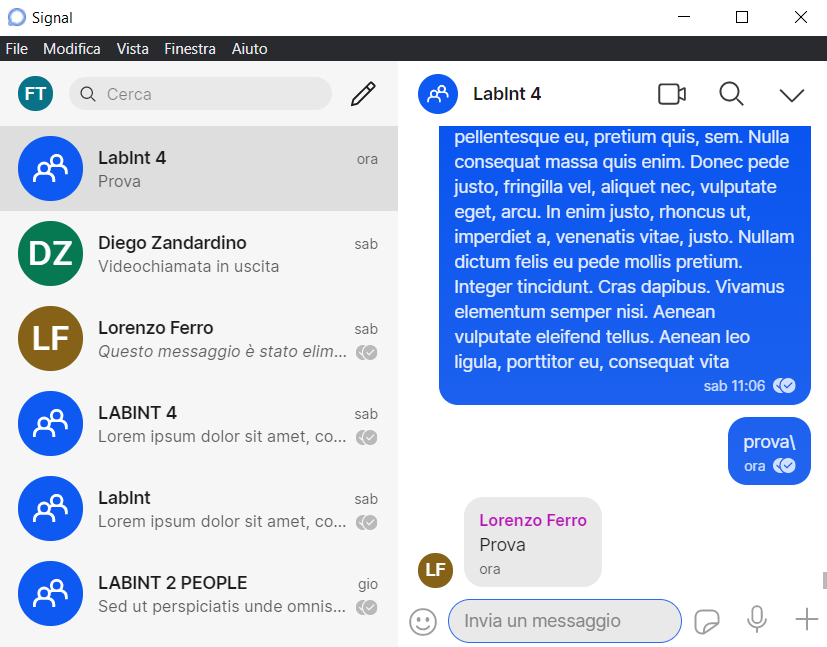
\includegraphics[scale=0.65]{interfaccia.png}
   \end{center}

   \pagebreak
   
   \section{Testbed}
   \begin{center}
    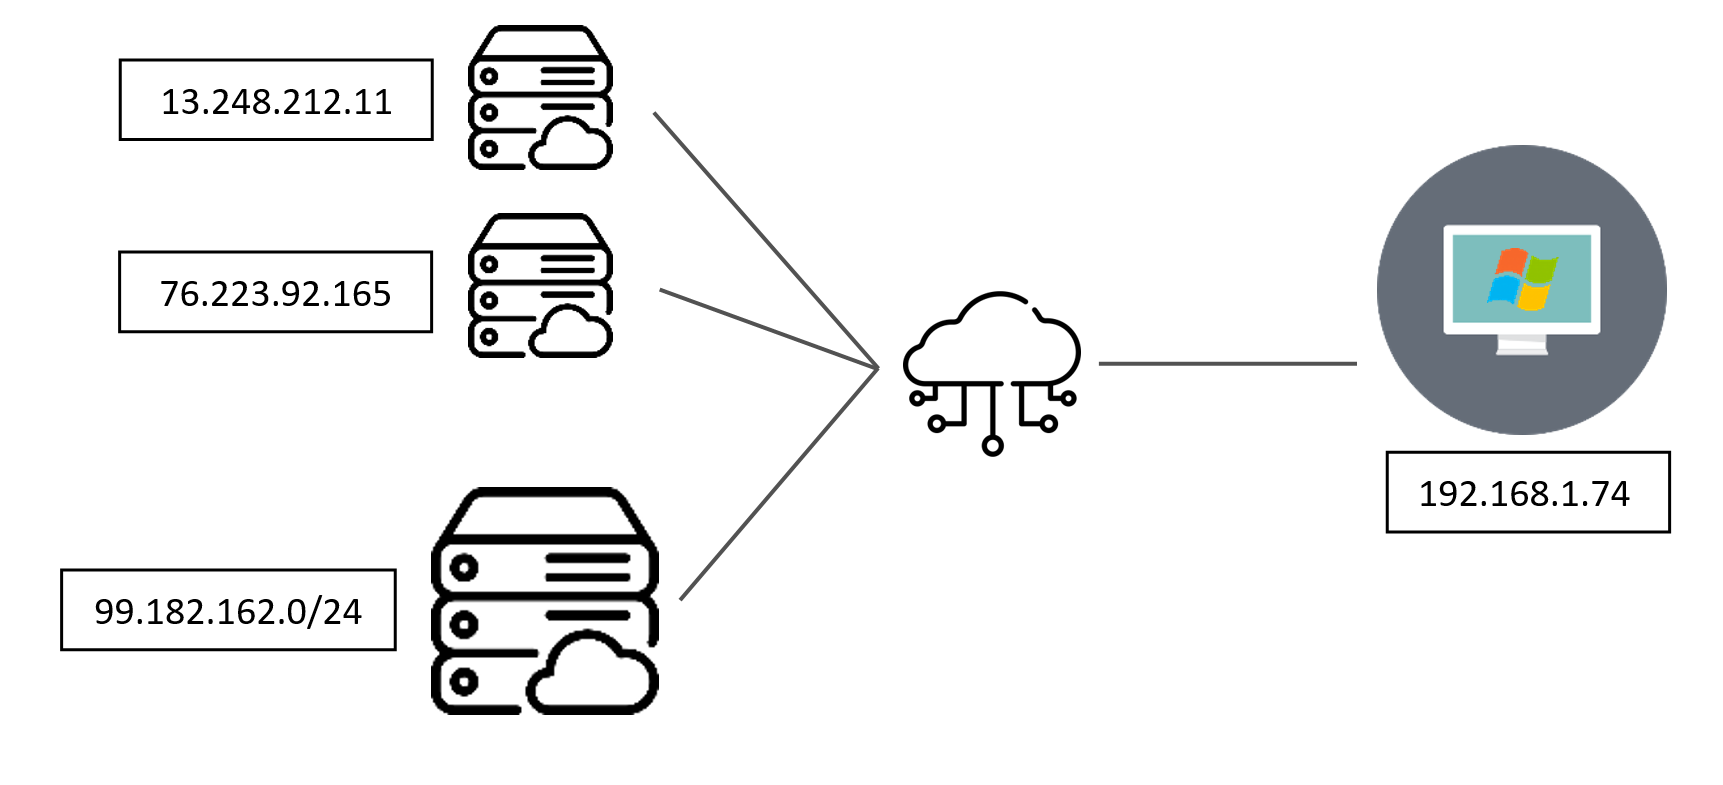
\includegraphics[scale=0.2]{testbed.png}
\end{center}

Per le analisi che abbiamo effettuato, si è utilizzato principalmente un computer Windows 10 (collegato
   tramite WiFi) con indirizzo ip \textit{192.168.1.74}, in altri scenari
   abbiamo utilizzato anche altri computer appartenenti a sottoreti diverse per confrontare i dati tra quelli che venivano inviati al server e quelli che 
   arrivavano al destinatario.\\
   Eseguendo il comando \textit{host www.signal.org} otteniamo il seguente output:\\
   \vspace{-20pt}
   \begin{verbatim}
 www.signal.org has address 13.226.175.98
 www.signal.org has address 13.226.175.88
 www.signal.org has address 13.226.175.31
 www.signal.org has address 13.226.175.56
   \end{verbatim}
   \vspace{-20pt}
   Questi risultati fanno però riferimento al sito web di signal e non coincidono interamente con quelli 
utilizzati dall'applicazione.
Si nota, attraverso le catture wireshark, che i server utilizzati dall'applicazione desktop a cui sono inviate le nostre richieste 
sono in realtà solo \textit{76.223.92.165 } e \textit{13.248.212.111}, quindi solo il secondo appartiene alla stessa 
sottorete degli indirizzi sopra elencati.
Analizzando gli indirizzi ip con l'ausilio di internet, si scopre che entrambi i server sono di proprietà Amazon 
e hanno apparentemente sede a Seattle (US). In realtà effettuando un ping a questi inidirizzi, entrambi ripsondono con un 
\textit{round-trip-time} di 20 ms, non compatibile con con i tempi che realmente un pacchetto impiegerebbe 
per percorrere la tratta Torino/Seattle/Torino. \\
Durante le analisi e la stesura della relazione ci siamo accorti che vengono utilizzati altri server, sempre di proprietà di amazon (servizio AWS) con sottorete 99.182.162.0/24,
che vengono interpellati quando la dimensione dei pacchetti inviati supera una certa dimensione. Nel grafico in Figura \ref{ServChan} vengono riportati in colore viola i Bytes 
ricevuti dai server \textit{76.223.92.165 } e \textit{13.248.212.111}, mentre in verde i Bytes/s ricevuti da un server nella sottorete 99.182.162.0/24. Inviando 4 messaggi
di dimensione crescente di nota che i primi due cioè i più piccoli sono inviati dai primi due server, mentre i due più grandi sono inviati dall'altro server, nonostante
i primi due continuino a mandare pacchetti probabilmente destinati al controllo della conversazione. \\ 
\begin{figure}[h]
  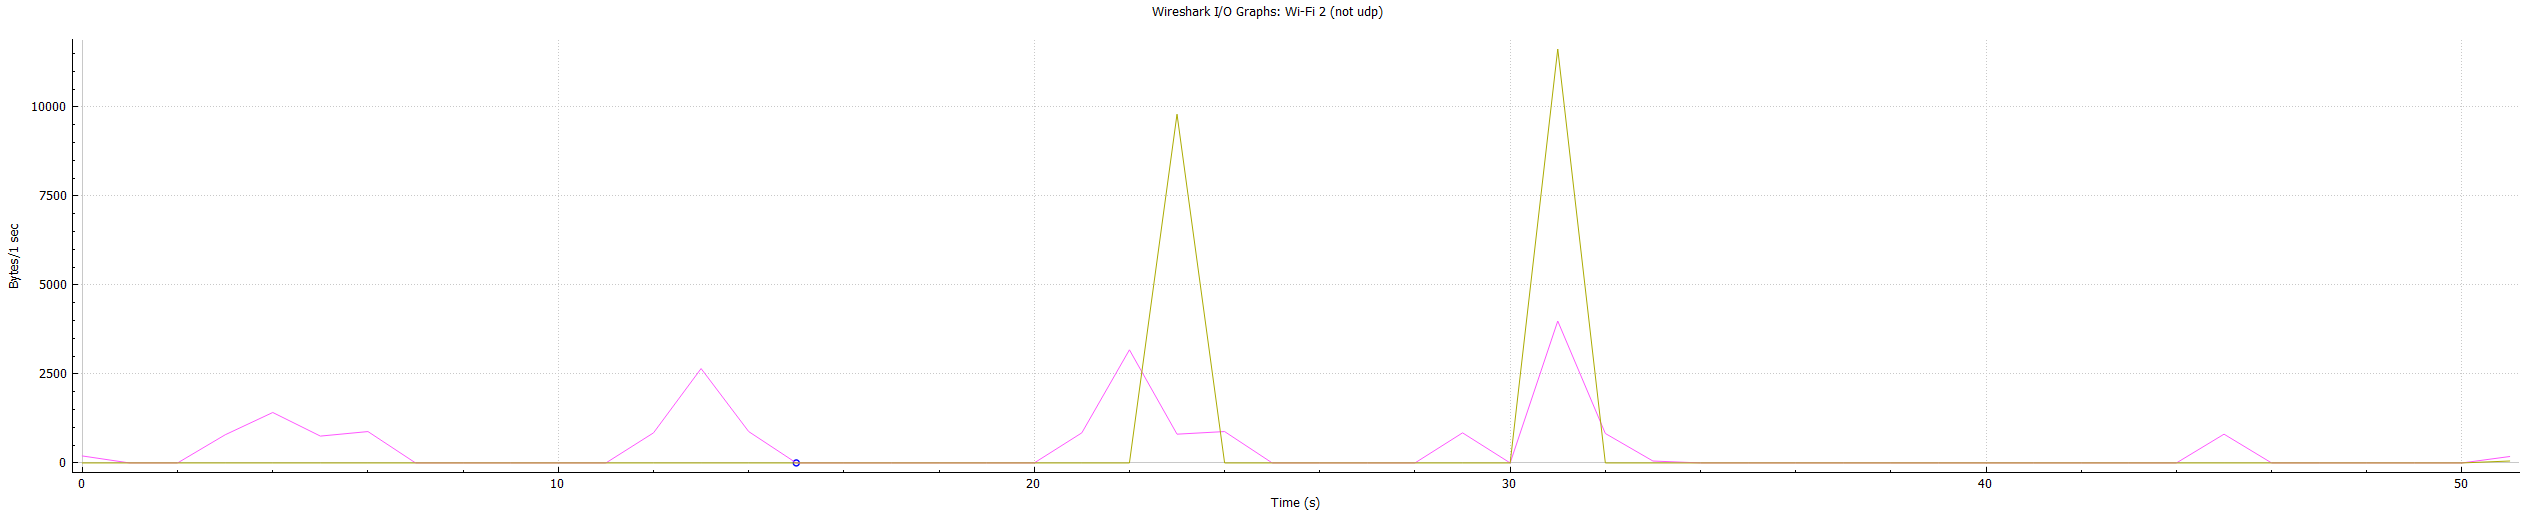
\includegraphics[width=1\textwidth]{serverChanges.png}
  \vspace{-20pt}
  \caption{Cambiamento server}\label{ServChan}
\end{figure}

Questo fatto può essere parzialmente spiegato siccome il servizio AWS non assegna staticamente i propri indirizzi ma adegua gli indirizzi
assegnati ai propri clienti a seconda della congestione, durante le analisi effettuate compaiono diversi inidirizzi ip appartenenti alla sottorete sopracitata.

Esegendo il comando traceroute con ciascuno dei seguenti indirizzi, non si hanno informazioni aggiuntive oltre al default gateway del router, 
tutti i pacchetti vanno in timeout senza ottenere risposta dai router intermedi.

\section{Apertura e chiusura app}

\begin{figure}[!htb]
  \begin{minipage}{0.3\textwidth}
      \centering
      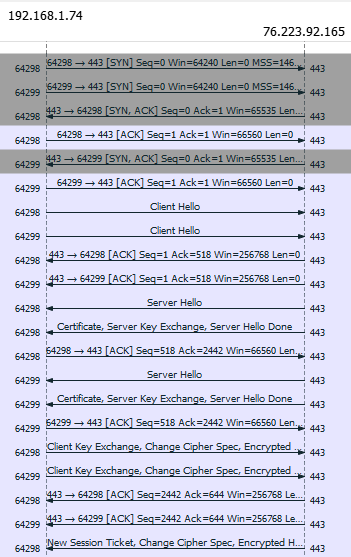
\includegraphics[width=0.9\linewidth]{flusso1.png}
      %\vspace{-20pt}
      \caption{Flusso prima parte}\label{flux1}
  \end{minipage}\hfill
  \begin{minipage}{0.3\textwidth}
      \centering
      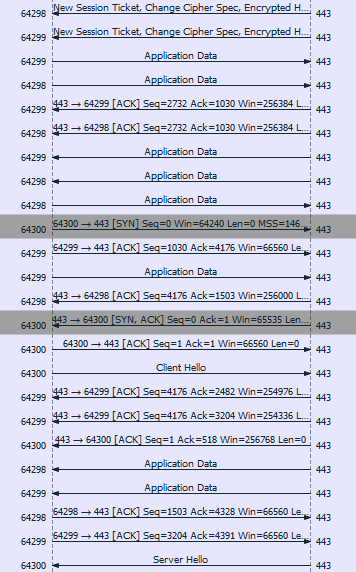
\includegraphics[width=0.9\linewidth]{flusso2.png}
      %\vspace{-20pt}
      \caption{Flusso seconda parte}\label{flux2}
  \end{minipage}\hfill
  \begin{minipage}{0.3\textwidth}
    \centering
    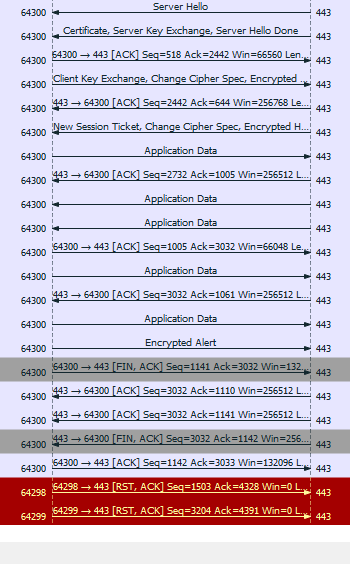
\includegraphics[width=0.9\linewidth]{flusso3.png}
    %\vspace{-20pt}
    \caption{Flusso terza parte}\label{flux3}
\end{minipage}\hfill
\end{figure}

In primo luogo si analizza il comportamento dell'applicazione all'avvio della stessa. 
Analizzando il traffico generato con Wireshark e ripetendo il test più volte è possibile 
riconoscere un protocollo di apertura e chiusura come segue:

\begin{itemize}
  \item TCP Three-Way-Handshake, ripetuta verso il server usando tre porte differenti
      \begin{itemize}
    \item TCP SYN
    \item TCP SYN, ACK
    \item TCP ACK
  \end{itemize}
    \item TLS v1.2 handshake, composta principalmente da: 
      \begin{itemize}
        \item \textit{Client Hello}: messaggio di apertura connessione del client verso il server, 
        in questo messaggio il client propone al server la versione di TLS 
        da utilizzare, la suite di cifratura che include gli algoritmi di 
        cifratura supportati e una stringa di bytes random (client-random)
        \item \textit{Server Hello}: in risposta al messaggio del client il server manda un 
        messaggio contenente il certificato SSL, la suite di 
        cifratura scelta dal server e un'ulteriore stringa di 
        byte random (server-random)
        \item Autenticazione e creazione della chiave di sessione attraverso lo scambio
        delle rispettive chiavi pubbliche (di client e server) e riscontro 
        con un messaggio criptato utilizzando la rispettiva chiave privata. 
        \begin{itemize}
          \item[$\Rightarrow $] scambio di Application Data e keep alive (filtrati in Figura \ref{flux1}, \ref{flux2} e \ref{flux3} )  della connessione
        \end{itemize}
        \item Encrypted Alert: mandato dal protocollo TLS per chiudere la connessione cifrata 
        quando non vi sono più dati da scambiare.
      \end{itemize}
      \item Chiusura connessione TCP 
      \begin{itemize}
        \item FIN, ACK
        \item ACK
        \item RST, ACK
      \end{itemize}
\end{itemize}

\pagebreak

\section{Messaggi}

\subsection{Privati}

\begin{wrapfigure}{r}{0.6\textwidth}
  \begin{center}
      \vspace{-20pt}
    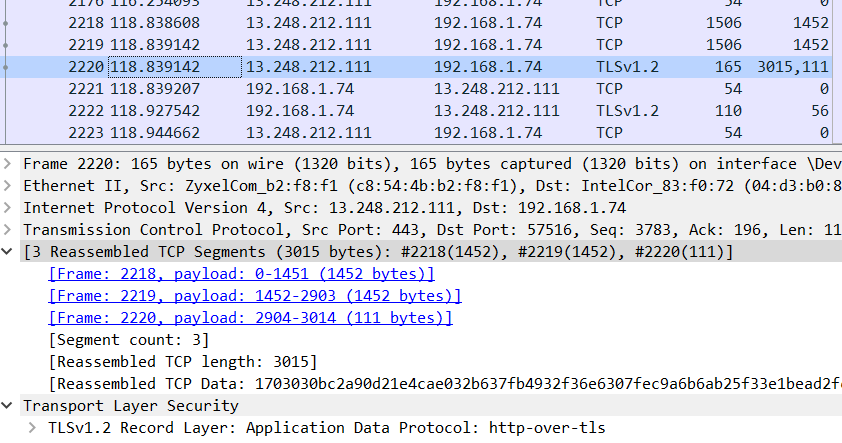
\includegraphics[width=0.58\textwidth]{framm.png}
  \end{center}
  \vspace{-20pt}
  \caption{Frammentazione TLS}
  \vspace{-10pt}
\end{wrapfigure}

Vediamo in seguito di analizzare il traffico generato dall'applicazione 
quando vengono scambiati messaggi in una chat privata. 
Per analizzare esaustiavemente il comportamento dell'applicazione si mandano diversi 
messaggi di dimensione crescente. Si nota che il protocollo TCP esegue frammentazione 
per pacchetti di dimensione superiore ad una MTU (1452 Byte) ma questi
vengano racchiusi in un unico pacchetto TLS che si occupa di riassemblare
il payload. Come accennato nell'introduzione prendendo in considerazione il grafico in Figura \ref{ServChan},
abbiamo notato che per pacchetti di dimensione maggiore di 3015 Bytes vengono usati i server con rage di indirizzi 99.182.162.0/24.
Questi server sono utilizzati solo per mandare pacchetti contenti i dati del messaggio, mentre gli altri due (\textit{76.223.92.165 } e \textit{13.248.212.111})
mantengono la loro funzione scambiando messaggi di controllo.\\ 

Durante la conversazione sono mandati diversi pacchetti per migliorare 
l'esperienza utente. Dopo diversi test si può ipotizzare che l'applicazione mandi i seguenti pacchetti:

\begin{itemize}
  \item un pacchetto (di dimensione che varia da mittente a destinario) per avvisare uno dei due host che l'altro sta digitando dei caratteri nella casella di testo. 
  Se l'utente continua a digitare l'informazione è aggiornata mandando un pacchetto ogni 10 secondi, altrimenti è mandato un pacchetto 
  quando l'host termina di digitare. 
  \item un pacchetto (di dimensione che varia da mittente a destinario) per avvisare dell'avvenuta ricezione del messaggio da parte del destinatario.
  \item un pacchetto (di dimensione che varia da mittente a destinario) per avvisare della lettura del messaggio da parte del destinatario. 

\end{itemize}

L'applicazione permette inoltre di disabilitare l'indicatore di scrittura e la conferma di lettura; entrambe queste modifiche sono 
visibili nella cattura come un numero ridotto di informazioni aggiuntive scambiate (questa impostazione ci ha permesso di 
identificare le probabili dimensioni dei pacchetti sopra elencati, che abbiamo riportato in appendice in tabella).
\\
\'E importante notare che c'è una differenza nelle dimensioni dei pacchetti di segnalazione tra mittente e destinatario.
Infatti quando il mittente sta digitando vengono mandati al server pacchetti di lunghezza 787 Bytes, mentre il destinatario 
riceve pacchetti di lunghezza 791 Bytes. In risposta a questi messaggi si è notato che il server manda pacchetti di dimensione 
rispettivamente 269 Bytes e 110 Bytes che presumibilmente sono dei messaggi di controllo a livello applicazione, con una funzione
simile agli ACK TCP ma a un livello differente della pila protocollare.

\begin{figure}[h]
  \centering
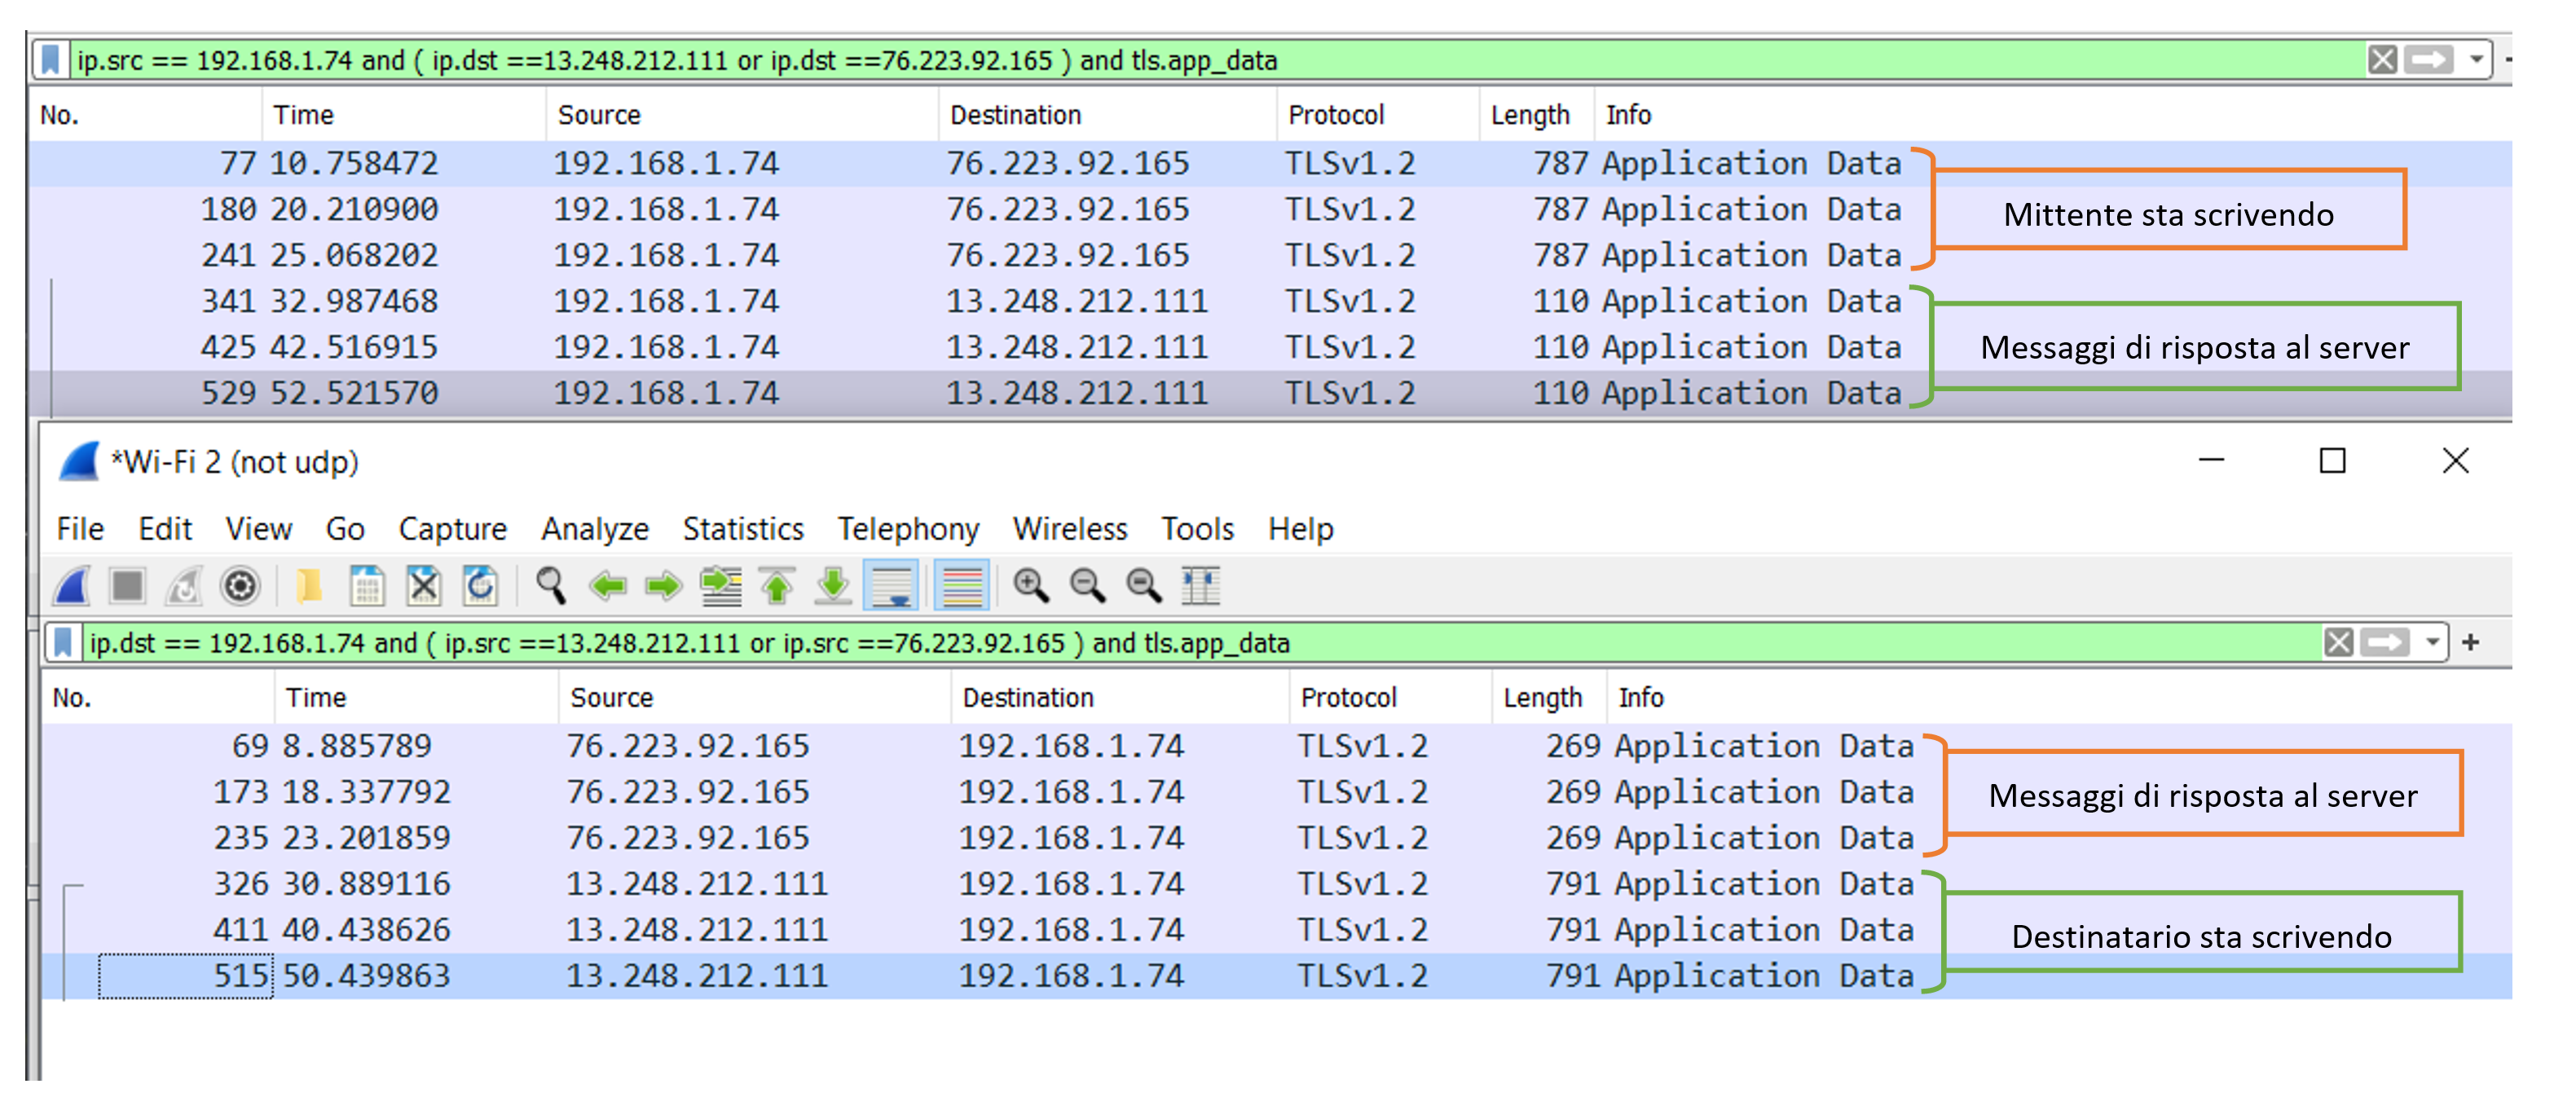
\includegraphics[width=0.8\textwidth]{mittDest.png}
\vspace{-20pt}
\caption{Mittente Destinatario}\label{mitDest}
\vspace{-20pt}
\end{figure}


\subsection{Gruppi}

% Prima di analizzare il traffico generato scambiando dei messaggi sui gruppi e' bene far notare che signal
% non tinene in memoria nei propri server i dati riguardanti ai gruppi e i suoi partecipanti. Proprio per questo ci 
% aspettiamo che i a livello applicazione e' come se ogni messaggio fosse mandato singolarmente a ogni componente del 
% gruppo. 

Dalle catture effettuate si nota come le dimensioni dei pacchetti scambiate nei gruppi sono significativamente più grandi 
rispetto a quelle di uno stesso messaggio in una chat privata. Le dimensioni dei pacchetti crescono poi in maniera poco 
significativa al crescere del numero degli utenti del gruppo, questo probabilmente per i meccanismi usati dall'applicazione per 
la gestione dei gruppi. \'E ragionevole pensare che in aggiunta al contenuto del messaggio, vi siano ulteriori Byte che contengono 
le informazioni relative al gruppo ed ai suoi membri. Nel grafico in Figura \ref{grup5} è rappresentata la quantità di Byte scambiata in 
funzione del tempo rispettivamente per:
\begin{itemize}
  \item[I)] chat singola
  \item[II)] chat di gruppo composta da 3 persone
  \item[III)] chat di gruppo composta da 4 persone
  \item[IV)] chat di gruppo composta da 5 persone
\end{itemize}

\begin{figure}[h]
  \centering
  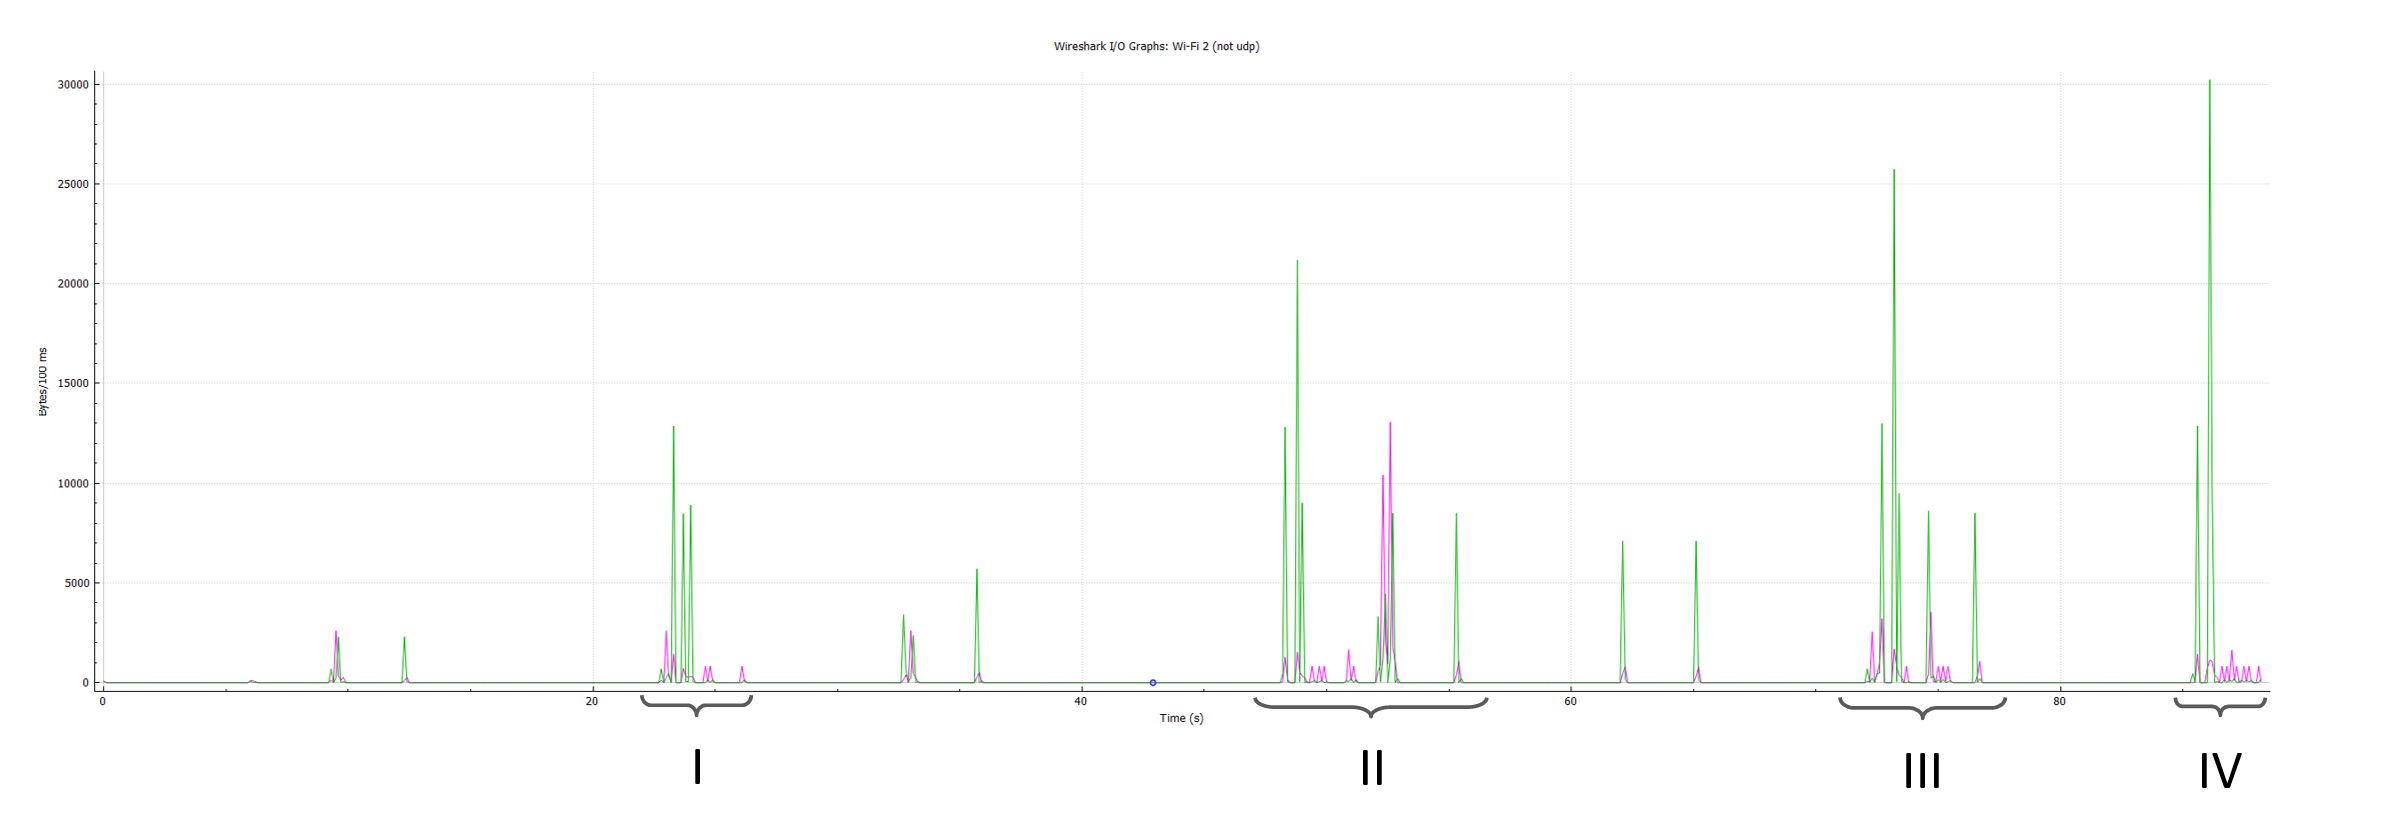
\includegraphics[width=1\textwidth]{5gruppi.png}
  \caption{Confronto gruppi con fino a 5 partecipanti}\label{grup5}
  \end{figure}

L'incremento dovuto all'intestazione all'interno dei gruppi rispetto alla chat privata si può notare in Figura \ref{grup5}, 
dove sono rappresentati in verde i Bytes/s inviati dall'host che effettua la cattura al server, e in viola i Bytes/s che esso riceve.

\begin{figure}[h]
  \centering
  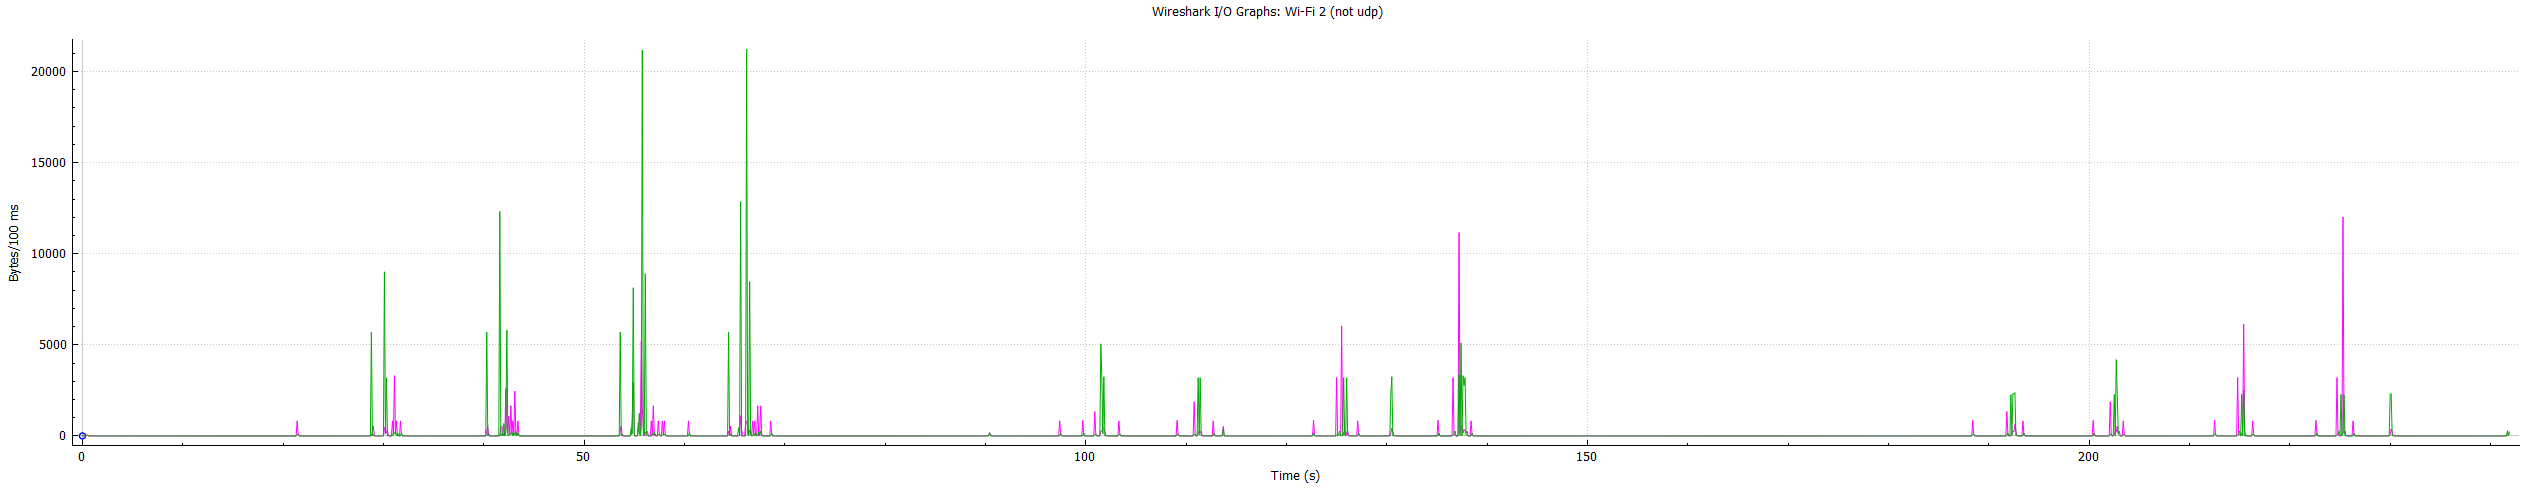
\includegraphics[width=1\textwidth]{PacchettiMandVsRic.png}
  \caption{Pacchetti mandati in relazione a ricevuti}\label{MandVsRic}
  \end{figure}

  Il grafico in Figura \ref{MandVsRic} mostra i pacchetti generati quando ogni partecipante di un gruppo composto da 3 utenti manda
  quattro diversi messaggi di dimensione crescente in diversi intervalli di tempo. Nel primo intervallo di tempo è l'utente che esegue 
  la cattura wireshark a mandare i messaggi, ed è possibile distinguere in viola il totale dei Byte al secondo ricevuti e in verde quelli 
  mandati. Nei due intervalli di tempo successivi sono invece gli altri partecipanti del gruppo a scrivere.
  \'E possibile notare la differenza tra i Byte mandati e ricevuti in qualità di mittente e destinatario, perchè il destinatario risponde 
  con informazioni riguardanti l'avvenuta cosegna o lettura del messaggio. Si può inoltre ipotizzare che la differenza 
  tra i Byte mandati nel primo intervallo e quelli ricevuti negli intervalli successivi sia dovuta a intestazioni e informazioni di controllo generati a
  livello applicativo.



\pagebreak

\subsection{Vocali e Multimediali}
Analizzando il traffico dopo aver mandato messaggi vocali o multimediali, abbiamo notato che vengono utilizzati solo i server compresi nella sottorete
99.182.162.0/24, mentre si inviano messaggi di controllo sempre con \textit{76.223.92.165 } e \textit{13.248.212.111}. 
L'invio dei pacchetti avviene sempre tramite lo stesso meccanismo dei messaggi, con connessione e pacchetti crittografati, facendo uso del protocollo
TCP e TSL.\\\\
Riportiamo di seguito due grafici riferiti all'invio di un file video di dimensione pari a 88MB.
\vspace{10pt}
\begin{figure}[!htb]
  \begin{minipage}{0.48\textwidth}
      \centering
      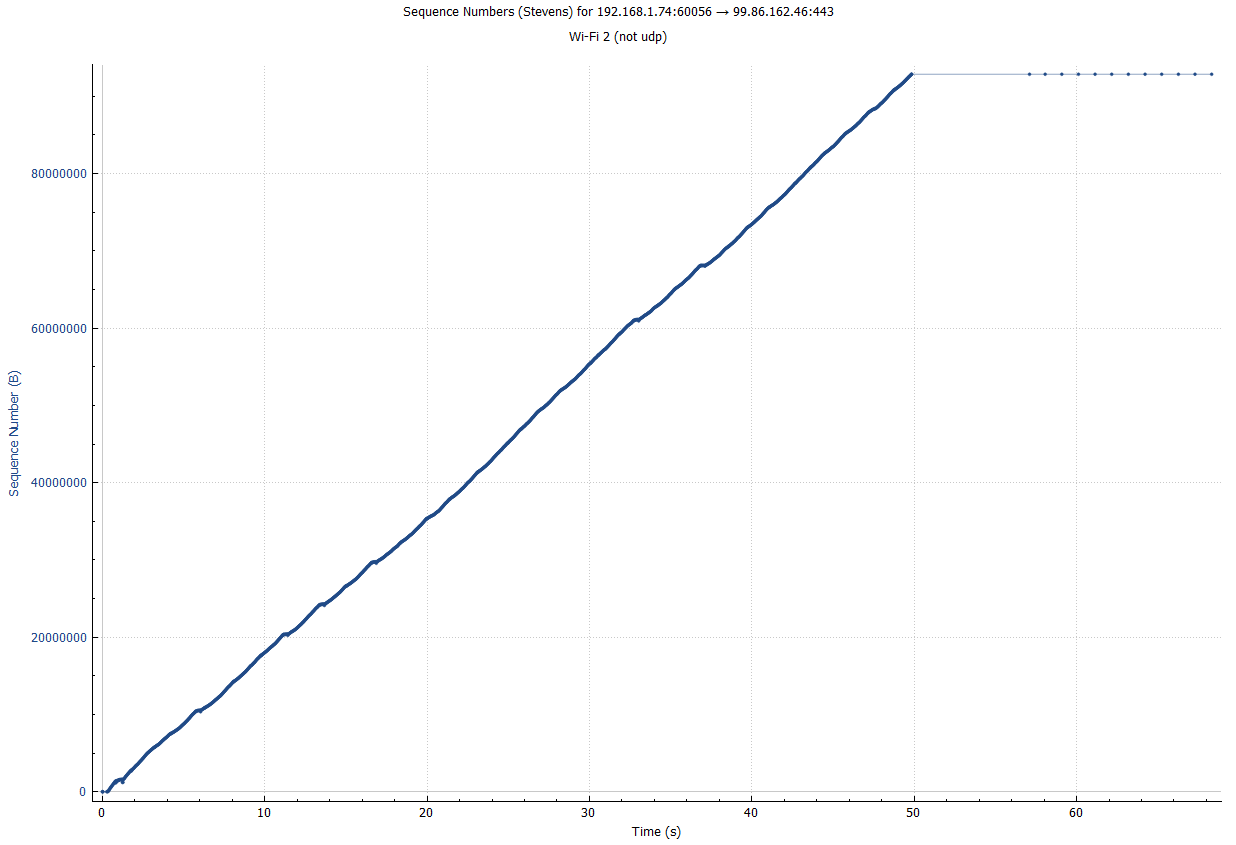
\includegraphics[width=1\linewidth]{filestevens.png}
      \vspace{-20pt}
      \caption{TCP STEVENS}\label{STEVENS}
  \end{minipage}\hfill
    \begin{minipage}{0.48\textwidth}
        \centering
        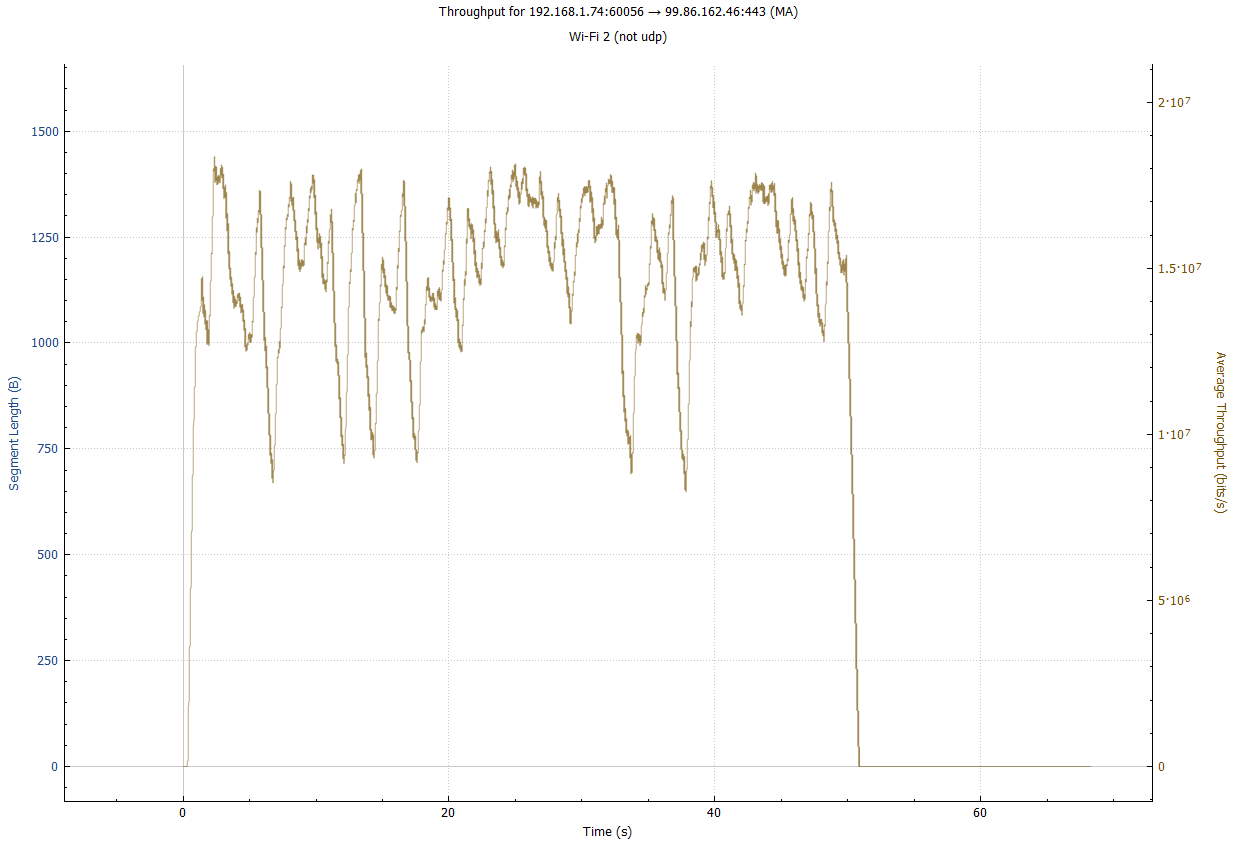
\includegraphics[width=1\linewidth]{filethr.png}
        \vspace{-20pt}
        \caption{TCP THROUGHPUT}\label{THROUGHPUT}
    \end{minipage}\hfill
  \end{figure}

  Ipotizzando che la connessione al server sia almeno 1Gb/s, non ci aspettiamo particolari problemi nella trasmissioni TCP causati da bottleneck.
  Nel grafico in Figura \ref{THROUGHPUT} si evidenzia che il throughput rimane abbastanza costante considerando che durante il test è stata utilizzata 
  una connessione con velocità di upload di circa 20MB/s. 
  Nel grafico in Figura \ref{STEVENS} si possono notare alcune ritrasmissioni, trascurabili considendo il totale di pacchetti inviati,e
  l'andamento complessivo quindi è lineare.\\\\
  
  I messaggi vocali assumono lo stesso comportamento dei file multimediali, 
  probabilmente perchè sono considerati come file audio nel momento dell'invio.

  \section{Videochiamate}

  In Figura \ref{testbed2} è riportato lo scenario che rapprensenta la videochiamata tra due utenti Signal.

  \begin{figure}
  \begin{centering}
    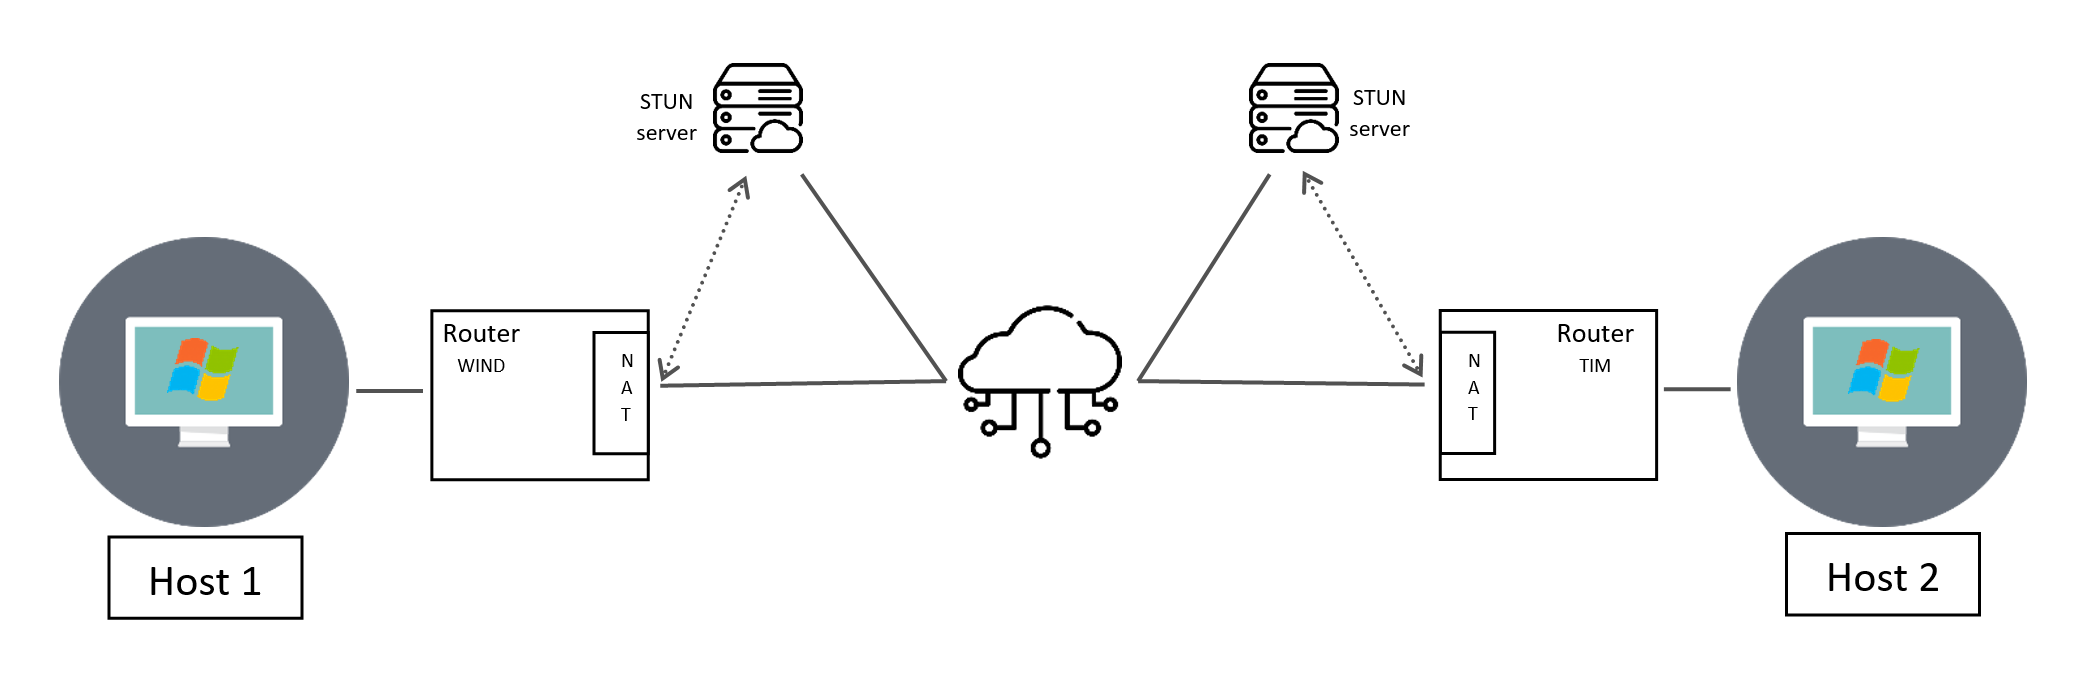
\includegraphics[width=1\linewidth]{testbed2.png}
    \caption{Testbed Videochiamate}\label{testbed2}
  \end{centering}
\end{figure}
\pagebreak

  \vspace{-10pt}
  \begin{figure}[!htb]
    \begin{minipage}{0.48\textwidth}
        \centering
        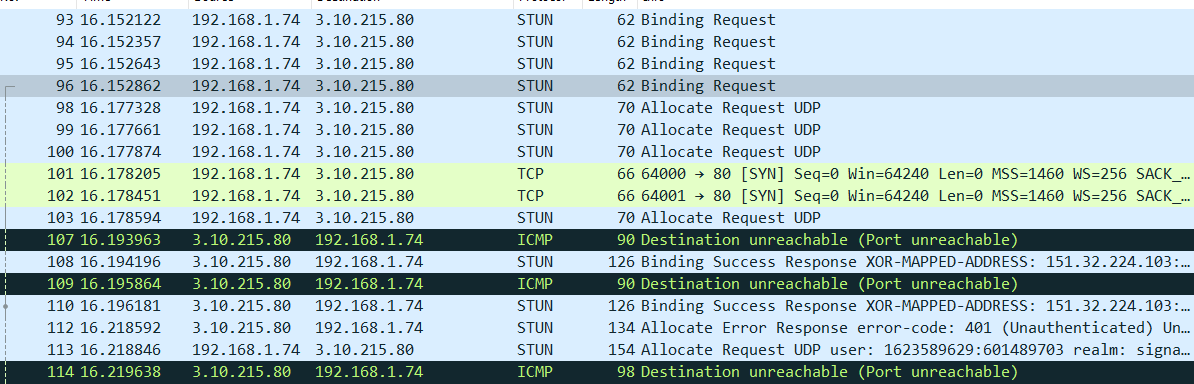
\includegraphics[width=1\linewidth]{chiamatacnn1.png}
        \vspace{-20pt}
        \caption{Apertura connessione}\label{conopen}
    \end{minipage}\hfill
      \begin{minipage}{0.48\textwidth}
          \centering
          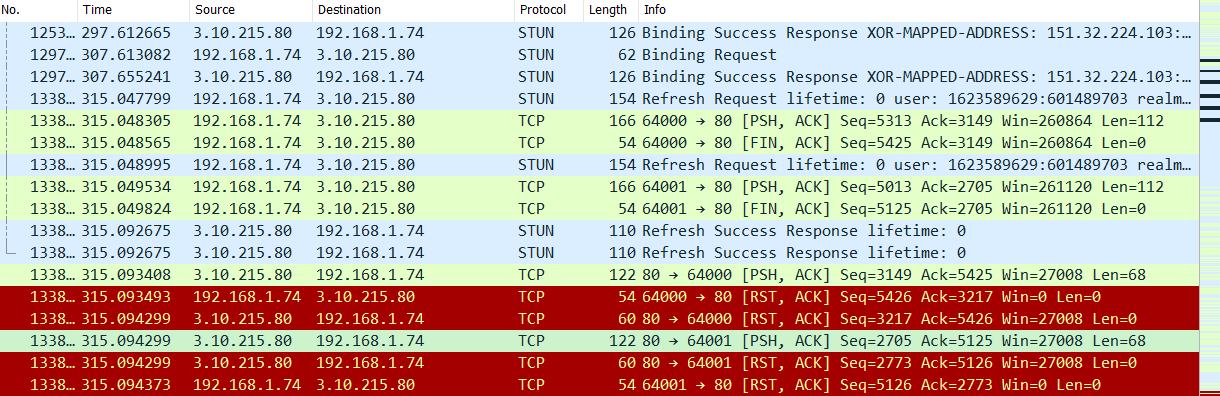
\includegraphics[width=1\linewidth]{chiamatacnn2.png}
          \vspace{-20pt}
          \caption{Chiusura connessione}\label{conclose}
      \end{minipage}\hfill
    \end{figure}

    
    Per concludere l'analisi di tutte le funzionalità offerte dall'applicazione 
    resta da osservare il suo comportamento durante le videochiamate. A differenza dei casi precedenti è ragionevole 
    ipotizzare che per questo tipo di servizio sia utilizzato il protocollo UDP, sfruttato a livello applicazione 
    da protocolli quali RTP e RTCP\footnote{[RFC 3550]}.
    In apertura della videochiamata si nota subito come venga utilizzato il protocollo
    STUN \footnote{Il protocollo STUN [RFC 5389] è un protocollo client-server che permette
    di sfruttare la tecnologia Voip, otennedo informazioni su NAT e firewall
    presenti tra il computer e la rete pubblica. Tramite il protocollo UDP si mette in
    comunicazione con il client STUN (implementando inoltre un trasferimento affidabile) per
    venire a conscenza dell'indirizzo pubblico utilizzato dal NAT, e permettere così la 
    comunicazione con un host nella rete pubblica, facendo uso della rete di server STUN esistenti.}.
    Eseguendo il comando \textit{whois} degli indirizzi utilizzati durante la videchiamata si ottiene un 
    risultato inatteso:
    un primo utente utilizza un indirizzo appartenente ad una sottorete posseduta da Telecom Italia (Tim), 
    mentre l'altro un indirizzo appartente ad una sottorete di proprietà Wind. Questi due altro non sono che gli 
    internet service provider dei due utenti che hanno effettuato i test. In particolare l'utente TIM si collega con
    un server Wind che ha indirizzo IP corrispondendente all'indirizzo pubblico assegnato al modem
    dell'interlocutore 
    per mettersi in comunicazione con l'altro host (che ha WIND come ISP) e viceversa. \\
    
    
    \begin{figure}[h]
      \centering
      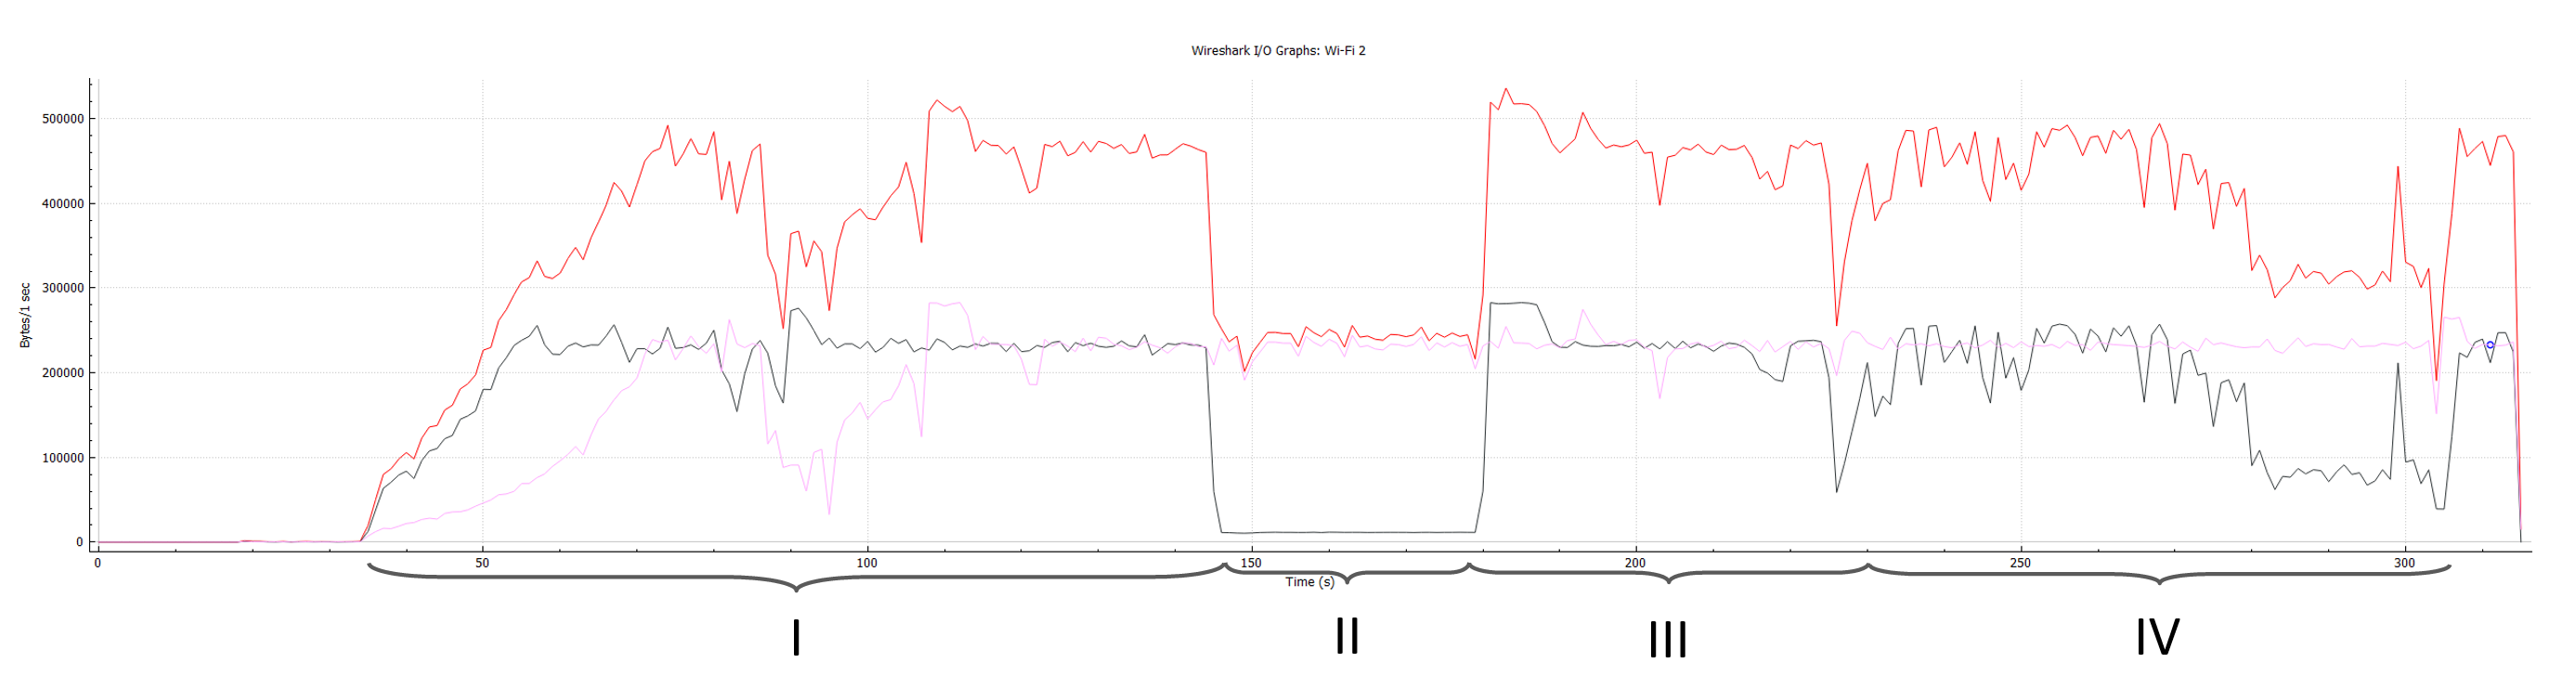
\includegraphics[width=1\textwidth]{chiamata.png}
      \caption{throughtput}\label{thr}
    \end{figure}
    
    Per analizzare esaustiavemente lo scenario in esame è stato eseguito un test che tenesse
    conto di tutte le proprietà di una videochiamata. Analizzando la Figura \ref{thr}, che raffigura in rosa il traffico inbound, in nero 
    il traffico outbound e in rosso quello totale, si notano diverse variazioni del throughput, causate dalle seguenti varizioni:
    \begin{itemize}
      \item[I)] in questo intervallo [ 35s - 150s ] i due host hanno sia microfono che videocamera accesi. L'host che genera il traffico in arrivo (in rosa avrà la stessa configurazione per tutto il test). Il calo di prestazione del destinatario che si nota in questo intervallo è dovuto ad un calo delle performance della rete. 
      \item[II)] in questo intervallo [ 150s - 175s ] l'host che esegue la cattura disabilita la videcamera riducendo ad un ventesimo dell'intervallo precedente il traffico generato. Come si poteva intuire questa modifica è quella che più impatta il traffico totale generato.
      \item[III)] in questo intervallo [ 190s - 210s ] è disattivato il microfono. Dopo un'iniziale variazione dovuta alla commutazione videocamera accesa - microfono spento, si nota che la differenza rispetto al primo intervallo è minima, seppur presente.
      \item[IV)] in quest ultimo intervallo [ 220s - 300s ] viene attivata la condivisione dello schermo, che di default disabilita la videocamera. il traffico generato è inferiore di quello nel primo intervallo, pur trattandosi di una condivisione real time di file video.
    \end{itemize}
    Tutto il traffico generato è composto da pacchetti RTP e controllato da RTCP, entrambi \textit{UDP-based}. 

    \subsection{Videochiamate di gruppo}
    \vspace{-10pt}

    Per le videochiamate di gruppo vengono utilizzati gli stessi protocolli delle videochiamate private tra due persone,
    però  tutti i membri della chiamata utilizzano lo stesso server (localizzato a Francoforte) per mandare e ricevere i pacchetti UDP, 
    sempre di proprietà di Amazon.

    \begin{figure}[h]
      \centering
      
      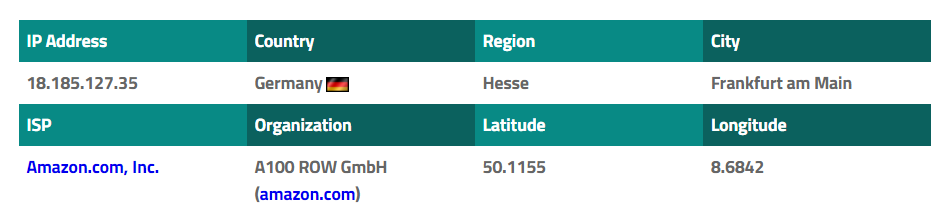
\includegraphics[width=0.8\textwidth]{francoforte.png}
      \vspace{-10pt}
      \caption{iplocation}\label{who}
    \end{figure}
    

  \section{Conclusioni}
  Il forte focus dell'applicazione da noi scelta sul garantire la privacy dei propri utenti salvando poche informazioni nei loro DataBase, 
  utilizzando algoritmi di cifratura e connessioni criptate end-to-end, e la caratteristica dei server Amazon di cambiare spesso i server utilizzati per
  le conversazioni, non ha reso l'analisi particolarmente semplice.\\
  Nonostante questo abbiamo rilevato dei comportamenti in gran parte prevedibili per un app di messaggistica, sicuramente sarebbero state di maggiore interesse
  capire i meccanismi di gestione degli header e delle informazioni scambiate a livello applicativo, ma ci è stato impossibile a causa dei protocolli 
  di crittografia. Abbiamo provato a trarre diverse conclusioni sulla base del tipo di messaggi inviati e sul fatto che molti messaggi di lunghezza fissa si ripetessero
  con una certa frequenza, ad esempio quelli che abbiamo considerato come dei messaggi a livello applicazione che avvisavano gli interlocutori che una determinata persona
  stesse scrivendo, stesse registrando un audio, avesse ricevuto o visualizzato un determinato messaggio. 
  Sarebbe stato, inoltre, interessante approfondire maggiormente come un messaggio criptato si modificasse in quanto a lunghezza e dimensione, ma non siamo riusciti
  ad estrarre queste informazioni con una semplice analisi tramite Wireshark.\\
  Molto interessante anche la funzionalità implementata per le chiamate di poter condividere lo schermo del dispositivo, per quanto riguarda l'applicazione Desktop per Windows 10, 
  inoltre in generale sembra avere una buona stabilità di connessione analizzando il throughput.\\
  Sicuramente dai test che abbiamo fatto possiamo concludere che Signal non ha nulla da invidiare alle altre applicazione di messaggistica, essendo utilizzatori quotidiani
  di Whatsapp e Telegram, e inoltre molto interessante per i più esperti
  che l'applicazione sia Open Source e il codice sia presente su GitHub consultabile in qualunque momento.

  \pagebreak
  
  \begin{appendices}
  \section{FILTRI WIRESHARK}
  \begin{verbatim}
    
  ip.dst == 192.168.1.74 and ( ip.src ==13.248.212.111 or ip.src ==76.223.92.165 
  or ip.dst  == 99.182.162.0/8 ) and tcp and not tcp.analysis.keep_alive and
  not tcp.analysis.keep_alive_ack
  

  ip.src == 192.168.1.74 and ( ip.dst ==13.248.212.111 or ip.dst ==76.223.92.165
  or ip.dst  == 99.182.162.0/8 ) and tcp and not tcp.analysis.keep_alive and 
  not tcp.analysis.keep_alive_ack

  \end{verbatim}
  \section{SERVER}
  \begin{verbatim}

  13.248.212.111
  76.223.92.165
  99.182.162.0/8

  \end{verbatim}

  \section{Lunghezze standard - Ipotizzate}

  I numeri riportati nelle prime due colonne della tabella sono le dimensioni dei pacchetti
  TLS.
  \begin{center}
    \begin{tabular}{|| c | c | c ||} 
    \hline
    H1 & H2 & Azione \\ [0.5ex] 
    \hline\hline
    787 & 269 & H1 \textit{sta scrivendo} a H2 \\ 
    \hline
    110 & 791 & H2 \textit{sta scrivendo} a H1 \\
    \hline
    110 & 827 & Conferma arrivo messaggio da H2  \\
    \hline
    110 & 829 & Lettura messaggio di H2 \\
    \hline
    123 & 124 & Keep Alive (sincronizzazione periodica) \\ 
    \hline
    187 & 110 & Richiesta di cancellazione di un messaggio \\ [1ex]
    \hline
   \end{tabular}
   \end{center}
  
  \end{appendices}
\end{document}


